% Chapter 8, Section 5

\section{Optimization Challenges \difficultyInline{intermediate}}
\label{sec:challenges}

Deep neural network optimization faces unique challenges including vanishing and exploding gradients, saddle points, and plateaus that require specialized techniques and careful hyperparameter tuning to overcome.

\subsection{Intuition: Why Training Gets Stuck}

Deep networks combine nonlinearity and depth, creating landscapes with flat plateaus, narrow valleys, and saddle points. Noise (SGD), momentum, and schedules act like navigational aids to keep moving and avoid getting stuck.\index{optimization!challenges}

\subsection{Vanishing and Exploding Gradients}

In deep networks, gradients can become exponentially small or large during backpropagation, creating fundamental challenges for training. Vanishing gradients occur when gradients become exponentially small as they propagate backward through the network, particularly common with sigmoid and tanh activation functions that have small derivatives. This phenomenon severely limits the ability of early layers to learn effectively, as their gradients become too small to drive meaningful parameter updates.

Exploding gradients represent the opposite problem, where gradients grow exponentially large during backpropagation, particularly common in recurrent neural networks due to the repeated application of the same weight matrices. These large gradients can cause parameter updates to become unstable, leading to training divergence or numerical overflow.

Modern deep learning addresses these challenges through several key techniques. ReLU activation functions, batch normalization, and residual connections help mitigate vanishing gradients by providing alternative pathways for gradient flow. Gradient clipping provides a direct solution to exploding gradients by limiting the magnitude of gradients during backpropagation. The mathematical formulation of gradient clipping rescales gradients when they exceed a threshold:

\begin{equation}
\vect{g} \leftarrow \frac{\vect{g}}{\max(1, \|\vect{g}\| / \theta)}
\end{equation}

where $\theta$ represents the clipping threshold. This approach prevents individual parameter updates from becoming too large while preserving the relative direction of the gradient vector.\index{gradient clipping}

\subsection{Local Minima and Saddle Points}\index{saddle point}

In high-dimensional optimization landscapes, saddle points are significantly more common than local minima, making them the primary challenge for gradient-based optimization methods. Saddle points represent critical points where the gradient is zero but the curvature is mixed, containing both positive and negative eigenvalues in the Hessian matrix. These points create deceptive flat regions where gradient descent can become trapped, as the zero gradient provides no directional information for escape.

The mathematical characterization of saddle points reveals their deceptive nature. At a saddle point, the gradient vanishes completely, but unlike local minima where all eigenvalues of the Hessian are positive, saddle points have mixed curvature with both positive and negative eigenvalues. This mixed curvature means that while some directions lead downhill (negative eigenvalues), others lead uphill (positive eigenvalues), creating a complex optimization landscape where simple gradient descent can become trapped.

Momentum and noise provide essential mechanisms for escaping saddle points in high-dimensional spaces. Momentum accumulates velocity from past gradients, providing sufficient inertia to overcome the zero gradient at saddle points and continue optimization. Stochastic noise from mini-batch sampling adds random perturbations that help the optimizer escape these deceptive flat regions by providing small random forces that can push the optimization trajectory away from saddle points.

\subsubsection{Example: Critical Points in Two Dimensions}

Consider the function $f(x,y) = x^4 - 2x^2 + y^2$ to illustrate different types of critical points. This function provides a clear example of how different critical points create distinct optimization challenges in the loss landscape.

\begin{figure}[h]
\centering
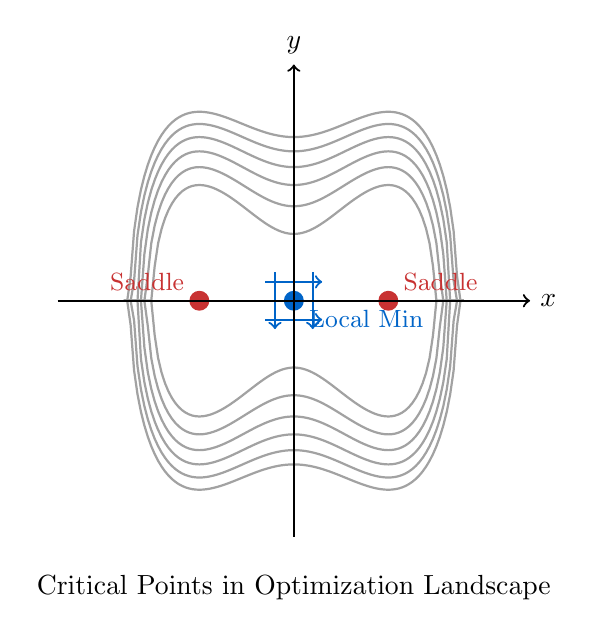
\begin{tikzpicture}[scale=1.2]
  % Define colors
  \definecolor{mincolor}{RGB}{0,100,200}
  \definecolor{saddlecolor}{RGB}{200,50,50}
  \definecolor{contourcolor}{RGB}{100,100,100}
  
  % Draw contour lines for the function f(x,y) = x^4 - 2x^2 + y^2
  \foreach \level in {0.5,1.0,1.5,2.0,2.5,3.0} {
    \draw[contourcolor!60, thick] plot[domain=-1.8:1.8, samples=100] (\x, {sqrt(max(0,\level - \x*\x*\x*\x + 2*\x*\x))});
    \draw[contourcolor!60, thick] plot[domain=-1.8:1.8, samples=100] (\x, {-sqrt(max(0,\level - \x*\x*\x*\x + 2*\x*\x))});
  }
  
  % Mark critical points
  % Local minimum at (0,0)
  \fill[mincolor] (0,0) circle (3pt) node[below right, xshift=2pt] {\small Local Min};
  
  % Saddle points at (±1,0)
  \fill[saddlecolor] (1,0) circle (3pt) node[above right, xshift=2pt] {\small Saddle};
  \fill[saddlecolor] (-1,0) circle (3pt) node[above left, xshift=-2pt] {\small Saddle};
  
  % Add arrows showing gradient directions
  \draw[->, mincolor, thick] (-0.3,0.2) -- (0.3,0.2);
  \draw[->, mincolor, thick] (-0.3,-0.2) -- (0.3,-0.2);
  \draw[->, mincolor, thick] (0.2,0.3) -- (0.2,-0.3);
  \draw[->, mincolor, thick] (-0.2,0.3) -- (-0.2,-0.3);
  
  % Add coordinate axes
  \draw[->, black, thick] (-2.5,0) -- (2.5,0) node[right] {$x$};
  \draw[->, black, thick] (0,-2.5) -- (0,2.5) node[above] {$y$};
  
  % Add labels
  \node[below] at (0,-2.8) {Critical Points in Optimization Landscape};
\end{tikzpicture}
\caption{Critical points in $f(x,y) = x^4 - 2x^2 + y^2$: minimum at $(0,0)$, saddle points at $(\pm 1,0)$.}
\label{fig:critical-points}
\end{figure}

The function $f(x,y) = x^4 - 2x^2 + y^2$ demonstrates three distinct types of critical points that commonly appear in optimization landscapes. At the local minimum $(0,0)$, the function value $f(0,0) = 0$ represents the lowest point in the neighborhood, with all nearby points having higher function values. The gradient vanishes at this point, and the Hessian matrix has positive eigenvalues, indicating concave-up curvature in all directions.

Saddle points at $(\pm 1,0)$ represent the most challenging critical points for optimization, where $f(\pm 1,0) = -1$ creates deceptive flat regions. These points have zero gradients but mixed curvature, with the Hessian containing both positive and negative eigenvalues. This mixed curvature means that while some directions lead downhill, others lead uphill, creating a complex landscape where gradient descent can become trapped.

In high-dimensional optimization, saddle points are much more common than local minima, making them the primary challenge for gradient-based methods. The visualization clearly shows how saddle points create deceptive flat regions where optimization can stall, while local minima provide clear convergence targets.

\subsection{Plateaus}\index{plateau}

Flat regions with small gradients slow convergence. Adaptive methods and learning rate schedules help navigate plateaus.

\subsection{Practical Optimization Strategy}

Developing an effective optimization strategy requires understanding the interplay between optimizer choice, learning rate scheduling, and problem-specific considerations. The recommended approach begins with Adam for rapid initial progress, using learning rates in the range $\{10^{-3},3\cdot10^{-4},10^{-4}\}$ to establish a strong foundation for training. This adaptive method provides robust performance across diverse architectures and datasets while requiring minimal hyperparameter tuning.

Learning rate scheduling plays a crucial role in optimization success, with different strategies suited to different model architectures. Cosine decay with warmup proves particularly effective for transformer-like models, providing smooth transitions from exploration to exploitation phases. For convolutional networks trained with SGD and momentum, step decay schedules often yield superior results by allowing the optimizer to make large initial progress before fine-tuning with smaller learning rates.

When validation accuracy saturates, switching from Adam to SGD with Nesterov momentum can improve generalization by providing different optimization dynamics. This transition requires careful tuning of both learning rate and momentum parameters, but often yields better final performance on vision tasks. Gradient clipping becomes essential in recurrent models and unstable training scenarios, preventing parameter updates from becoming too large while preserving optimization direction.

Continuous monitoring of training and validation metrics provides essential feedback for optimization strategy adjustment. Early stopping prevents overfitting by halting training when validation performance plateaus, while careful attention to learning rate schedules ensures optimal convergence behavior throughout the training process.\index{gradient clipping}\index{early stopping}

Applications and heuristics:
\begin{itemize}
    \item Vision: SGD+momentum or Nesterov often yields state-of-the-art with careful schedules and augmentations \cite{He2016}.
    \item NLP/Transformers: Adam/AdamW with warmup+cosine is a strong default; clip global norm in seq2seq models.
    \item Reinforcement learning: Adam with small $\alpha$ stabilizes non-stationary objectives.
\end{itemize}

Common failure modes:
\begin{itemize}
    \item Divergence at start: reduce $\alpha$, add warmup, or increase \(\epsilon\) for Adam.
    \item Plateau: try larger batch with warmup, use cosine schedule, or add momentum.
    \item Overfitting: increase regularization (weight decay, dropout), add data augmentation.
\end{itemize}
